% Copyright (C) 2014-2020 by Thomas Auzinger <thomas@auzinger.name>

% TODO add final option
\documentclass[draft, final]{vutinfth} % Remove option 'final' to obtain debug information.

% Load packages to allow in- and output of non-ASCII characters.
\usepackage{lmodern}        % Use an extension of the original Computer Modern font to minimize the use of bitmapped letters.
\usepackage[T1]{fontenc}    % Determines font encoding of the output. Font packages have to be included before this line.
\usepackage[utf8]{inputenc} % Determines encoding of the input. All input files have to use UTF8 encoding.

% Extended LaTeX functionality is enables by including packages with \usepackage{...}.
\usepackage{amsmath}    % Extended typesetting of mathematical expression.
\usepackage{amssymb}    % Provides a multitude of mathematical symbols.
\usepackage{mathtools}  % Further extensions of mathematical typesetting.
\usepackage{microtype}  % Small-scale typographic enhancements.
\usepackage{float}
\usepackage[inline]{enumitem} % User control over the layout of lists (itemize, enumerate, description).
\usepackage{multirow}   % Allows table elements to span several rows.
\usepackage{booktabs}   % Improves the typesettings of tables.
\usepackage{subcaption} % Allows the use of subfigures and enables their referencing.
\usepackage[ruled,linesnumbered,algochapter]{algorithm2e} % Enables the writing of pseudo code.
\usepackage[usenames,dvipsnames,table]{xcolor} % Allows the definition and use of colors. This package has to be included before tikz.
\usepackage{nag}       % Issues warnings when best practices in writing LaTeX documents are violated.
\usepackage{todonotes} % Provides tooltip-like todo notes.
\usepackage{hyperref}  % Enables cross linking in the electronic document version. This package has to be included second to last.
\usepackage[acronym,toc]{glossaries} % Enables the generation of glossaries and lists fo acronyms. This package has to be included last.
\usepackage{csvsimple}

% Define convenience functions to use the author name and the thesis title in the PDF document properties.
\newcommand{\authorname}{Tobias Schwarzinger} % The author name without titles.
\newcommand{\thesistitle}{Method Inlining in the Second Stage Compiler of the CACAO VM} % The title of the thesis. The English version should be used, if it exists.

% Set PDF document properties
\hypersetup{
    pdfpagelayout   = TwoPageRight,           % How the document is shown in PDF viewers (optional).
    linkbordercolor = {Melon},                % The color of the borders of boxes around crosslinks (optional).
    pdfauthor       = {\authorname},          % The author's name in the document properties (optional).
    pdftitle        = {\thesistitle},         % The document's title in the document properties (optional).
    pdfsubject      = {Subject},              % The document's subject in the document properties (optional).
    pdfkeywords     = {a, list, of, keywords} % The document's keywords in the document properties (optional).
}

\setpnumwidth{2.5em}        % Avoid overfull hboxes in the table of contents (see memoir manual).
\setsecnumdepth{subsection} % Enumerate subsections.

\nonzeroparskip             % Create space between paragraphs (optional).
\setlength{\parindent}{0pt} % Remove paragraph identation (optional).

\makeindex      % Use an optional index.
\makeglossaries % Use an optional glossary.
%\glstocfalse   % Remove the glossaries from the table of contents.

% Set persons with 4 arguments:
%  {title before name}{name}{title after name}{gender}
%  where both titles are optional (i.e. can be given as empty brackets {}).
\setauthor{}{\authorname}{}{male}
\setadvisor{Ao.Univ.Prof. Dipl.-Ing. Dr.techn.}{Andreas Krall}{}{male}

% For dissertations at the PhD School and optionally for dissertations:
\setsecondadvisor{Pretitle}{Forename Surname}{Posttitle}{male} % Comment to remove.

% Required data.
\setregnumber{11778257}
\setdate{26}{03}{2020} % Set date with 3 arguments: {day}{month}{year}.
\settitle{\thesistitle}{TBD} % Sets English and German version of the title (both can be English or German). If your title contains commas, enclose it with additional curvy brackets (i.e., {{your title}}) or define it as a macro as done with \thesistitle.

\setthesis{bachelor}
% For bachelor and master:
\setcurriculum{Software \& Information Engineering}{Software \& Information Engineering} % Sets the English and German name of the curriculum.

% For dissertations at the PhD School:
\setfirstreviewerdata{Affiliation, Country}
\setsecondreviewerdata{Affiliation, Country}


\usepackage[
backend=biber,
style=alphabetic,
citestyle=alphabetic
]{biblatex}
\addbibresource{references.bib}

\newrobustcmd*{\parentexttrack}[1]{%
  \begingroup
  \blx@blxinit
  \blx@setsfcodes
  \blx@bibopenparen#1\blx@bibcloseparen
  \endgroup}

\AtEveryCite{%
  \let\parentext=\parentexttrack%
  \let\bibopenparen=\bibopenbracket%
}

\usepackage{listings}

\lstset{
  frame=single,
  keywordstyle=\color{blue},
  language=Java,
  captionpos=b 
}

\begin{document}

\frontmatter % Switches to roman numbering.
% The structure of the thesis has to conform to the guidelines at
%  https://informatics.tuwien.ac.at/study-services

\addtitlepage{english} % English title page.

\begin{acknowledgements*}
First, I want to thank my family for always supporting me throughout my life. Without their financial and especially emotional support, none of this would be possible.

Furthermore, I want to thank Prof. Andreas Krall and the \textit{CACAO}-Team for giving me the chance to work on the \emph{CACAO} project and sharing their knowledge with me.

Last but not least I want to thank Carina and all my friends for helping me through the more rough phases of this work by always cheering me up and keeping me company.
\end{acknowledgements*}

\begin{kurzfassung}
\emph{Objektorientierte} Programmiersprachen fördern den Einsatz von Abstraktion (z.B. Methoden), um komplexe Probleme zu lösen. Programmierer tendieren dazu besser lesbaren und strukturierten Code zu schreiben, wenn sie ein großes Problem in mehrere einfache Subprobleme herunterbrechen. Inline-Ersetzung ist eine bekannte und effektive Optimierung, welche die Performanceeinbuße von Methodenaufrufen lindern. Zurzeit hat der Second-Stage-Compiler, \emph{Compiler2}, der virtuellen Maschine \emph{CACAO} keinen inliner. Das Ziel dieser Arbeit ist es einen neuen Compiler-Pass zu implementieren, welcher geeignete Methodenaufrufe findet und inlined, um die Gesamtperformance der virtuellen Maschine zu steigern.
\end{kurzfassung}

\begin{abstract}
An \emph{object-oriented} programming language promotes the use of \emph{abstraction} (e.g. methods) to tackle difficult tasks. By breaking down the problem into multiple simpler and smaller sub-problems, programmers tend to write more readable and structured code. Method inlining is a well-known and potent compiler optimization to mitigate the performance losses introduced by \emph{method calls}. Currently, the second stage compiler, \emph{Compiler2}, of the virtual machine \emph{CACAO} lacks an inliner, thus offering room for improvement. In this work a compiler pass was implemented, which identifies and inlines promising \emph{call sites} to improve the overall performance of the virtual machine.
\end{abstract}

% Select the language of the thesis, e.g. english or naustrian.
\selectlanguage{english}

% Add a table of contents (toc).
\tableofcontents % Starred version, e.g., \tableofcontents*, removes the self-entry.

% Switch to arabic numbering and start the enumeration of chapters in the table of content.
\mainmatter

\chapter{Introduction}

\section{Method inlining}

Method inlining is an optimization used by (\emph{just-in-time}) compilers operating on \emph{object-oriented} languages (e.g. \emph{Java}) or their respective intermediate language (e.g. \emph{Java Bytecode}). The main goals of this technique are to reduce the overhead introduced by method invocations and to provide further possibilities for other optimization techniques, as many of them only operate within the scope of a method.  As a result, method inlining reduces the need for complex interprocedural optimizations. Inlining a method is achieved by "copying" the body of the called method (\emph{callee}) to the \emph{caller} while replacing the original invoke instruction. In many cases, some transformations to the invoked method are required.

\section{Motivation}

The second stage compiler of the \emph{CACAO VM} \cite{Krall}, introduced by Josef Eisl in his master's thesis \cite{Eisl13}, currently lacks an inliner. As method inlining is an effective optimization to reduce the execution time of a program, \emph{Compiler2} needs an efficient inliner to compete with other just-in-time compilers. Furthermore, other optimizations, such as the constant propagation optimization introduced by Matthias Reisinger in \cite{Reisinger14}, will be more effective due to the increased method size.

\section{Aim of the work}

This work's goal is to add an inlining \emph{pass} to the new compiler framework. The implementation should be able to inline call sites with targets known at \emph{compile-time}. Furthermore, a guarded adaption of the algorithm should be created, which can be used to inline potentially polymorphic call sites. To prevent code explosion, the inliner should only optimize beneficial call sites. Therefore, a set of heuristics that guide the inliner should be developed in the course of this work.

\section{Structure of the work}

The second chapter will summarize promising approaches and technologies related to inline substitution. The third chapter will cover the implementation of the inliner, including problems and obstacles which slowed down or hindered the work. Additionally, it gives a brief overview of the \emph{Java Bytecode} instructions and the intermediate representation of \emph{Compiler2}. The fourth chapter will discuss the results of the evaluation, while the fifth and last chapter will give an outlook on possible improvements.

\chapter{State of the Art}
\label{sec:sota}

\section{General}

While many compiler optimizations almost always produce more efficient code, \emph{inlining} does not. Many factors play a role in whether it is beneficial to inline a particular \emph{call site}, and choosing these invocations is anything but trivial. The goal of an inliner is to find a balance between faster execution times, higher compilation times, and higher memory usage. The actual inlining algorithm, which copies the instructions from the \emph{callee} to the \emph{caller}, is highly specific to the \emph{intermediate representation} of the virtual machine; algorithms for finding beneficial \emph{call sites} are not. 

\begin{quote}
[...] any compilerwriter will tell you that inlining is a black art, full of delicate
compromises that work together to give good performance without unnecessary code bloat.\\
\cite[p.1]{Jones2002}
\end{quote}

Many different approaches try to maximize the benefits of method inlining. This chapter gives an overview of these techniques.

\section{Inlining techniques}
\label{sec:sota-techniques}

The actual inlining process is highly dependent on the specific \emph{intermediate representation} used by the compiler. Apart from implementation details, every inlining optimization copies instructions from the target method to the caller method, while applying some transformations to preserve the semantics of the program. Therefore, the original invocation will be replaced at least in some program paths. In simple cases only a small set of transformations are needed. For example, merely copying a \emph{return}-instruction, would result in a different control flow, thus potentially skipping instructions of the \emph{caller} method and producing an incorrect result.

If the target is not known at \emph{compile-time} (e.g. \emph{virtual} methods), the inliner has to take measures to ensure the program is still valid in all circumstances. The most straightforward solution is guarding the inlined code with a conditional statement. The most simple \emph{guard} is a \emph{class test}. While this ensures correct program execution, it does not minimize the number of executed \emph{virtual} calls in many cases. When two classes share the same method implementation (e.g. derived from a \emph{base} class), the inlined code will not get executed for one of the two classes\footnote{Assuming only a single \emph{class test} exists}. To address this problem, Detlefs and Agesen introduced \cite{Detlefs99} the concept of a \emph{method test}. If the invocation still refers to the same method in the current context, the \emph{method test} will succeed, thus allowing the processor to execute the guarded code. Arnold and Ryder \cite{Arnold02} suggested \emph{thin guards}, which reduce the overhead of \emph{guarded inlining} even further.

Even though modern processors eliminate a part of the overhead introduced by \emph{guarded inlining} by making use of \emph{branch-prediction}, they do not eliminate all overhead. Especially in scenarios with only one implementation loaded, thus reducing the polymorphic call to a monomorphic call, these checks are not necessary. For this reason, some compilers use \emph{devirtualization} in combination with optimistic \emph{assumptions}. This mechanism provides optimizations with the ability to register an assumption over the current state of the program (e.g. only one implementation of this virtual method is loaded). If any of these \emph{assumptions} break (e.g. by loading another class), the compiler \emph{recompiles} the method. Implementing such an approach poses many difficulties, especially the need for \emph{on-stack replacement}, because \emph{assumptions} may break when a method is currently active. Steiner already discussed this problem in the context of \emph{CACAO} in his master's thesis \cite{SteinerM07} in thorough detail.\emph{Preexistence-based inlining} is an option to eliminate the need for \emph{on-stack replacement} in some instances\cite{Detlefs99}.

\section{Knapsack based heuristics}
\label{sec:sota-knapsack}

Scheifler showed in his work \cite{Scheifler77}, that inline substitution is a \emph{intractable} problem, by reducing it to the well-known \texttt{KNAPSACK} problem. Noncoincidently, a popular way to model the creation of an \emph{inlining plan} is reducing it to the \texttt{KNAPSACK} problem, while a function determines the priority of \emph{call sites}. Solving the optimization-form of the \texttt{KNAPSACK} problem is known to be \texttt{NP-hard} \cite{Scheifler77}. As a single method can contain many method invocations, solving this problem optimally in a \emph{just-in-time} compiler could lead to high latency, due to increased compilation time. Fortunately, there are approximation algorithms. A simple, yet effective algorithm, proposed by Scheiffler \cite{Scheifler77}, chooses the next item with the highest benefit over cost ratio. This algorithm was already used in the \emph{CACAO} baseline compiler \cite{Steiner07} and the Jalapeño VM \cite{Arnold00}.

A straight forward way of calculating the costs of an inlining operation is merely counting the number of instructions in the callee method\footnote{including possible guard instructions}. By setting the benefit to $1$, one can reduce the number of variables needed to determine the priority of a \emph{call site}. Unfortunately, such simple heuristics will not perform as well as more sophisticated approaches. Davidson \emph{et al.} \cite{Davidson92} already suggested that the increase in code size should not be the only concern when constructing inlining heuristics. Arnold \emph{et al.} showed \cite{Arnold00} that \emph{inlining decisions} based on \emph{dynamic call graphs} yield better results compared to their static counterparts.

\section{Inlining Trials}

Many \emph{inlining heuristics} try to estimate the benefit and the cost of inlining a given \emph{call site} by analyzing the \emph{source code} (or \emph{intermediate representation}) of the target method. These estimations may not be close to the actual values, as a big part of the benefit may be created by subsequent optimization passes. Contrarily, an \emph{inlining decision} may result in high costs in a later pass (e.g. many register spills). Dean and Craig \cite{Dean94} proposed a method that tentatively performs \emph{inline expansion} and analyzes the result to determine the benefit and the cost of a given expansion. If the inliner concludes that this expansion is not advantageous, the transformation is reversed. The algorithm then stores the information in a \emph{persistent} database to avoid repeated executions of the \emph{inlining trial} at similar \emph{call sites}. Dean and Craig concluded that this approach yields overall faster compilation times and reduces the increase in code size while providing roughly the same execution speed.

\section{Incremental approaches}

To achieve better estimates for the actual benefit and cost, Prokopec \emph{et al.}\cite{Prokopec19} suggested incremental approaches to inlining. These algorithms alternate between expanding \emph{call sites} and applying other optimizations, thus giving the inliner more accurate data in the next iteration. They concluded that such an approach outperforms \emph{state-of-the-art} algorithms.

\section{Machine learning assisted heuristics}

Making the right inlining decisions is a complicated endeavour which depends on many variables. Sophisticated functions are needed to estimate the benefits and costs of a given \emph{call site}. Simon \emph{et al.} \cite{Simon13} suggested that using \emph{machine learning} can lead to high performing \emph{inlining heuristics}. In their work, they achieved significant speedups compared to manually crafted heuristics. 

\chapter{Implementation}

\section{Java Bytecode}

To implement \emph{method inlining}, one has to understand the different types of method invocations, the \emph{Java Virtual Machine Specification} describes. As of this work the \emph{CACAO VM} does not fully support JVMS\footnote{Java Virtual Machine Specification} SE 7 \cite{JVMSpec}. Therefore, the \texttt{invokedynamic} instruction will be ignored in the course of this work. The following enumeration introduces the remaining invoke instructions.

\begin{enumerate}
    \item \texttt{invokestatic} calls a \texttt{static} method (target is known at compile time).
    \item \texttt{invokespecial} calls an \texttt{<init>}, \texttt{private} or \emph{superclass} method (target known at compile time).
    \item \texttt{invokevirtual} calls a virtual method.
    \item \texttt{invokeinterface} calls a virtual method via an interface.
\end{enumerate}

\section{The intermediate representation}
\label{sec:intermediate_representation}

This section briefly discusses the structure and semantics of the \emph{high-level} intermediate representation, due to it being crucial for a complete understanding of the inliner. Additionally, some crucial notions and properties of this data structure will be discussed. For a more thorough description of the intermediate representation(s) consult \cite{Eisl13}. The second stage compiler in \emph{CACAO} uses two different intermediate representations of the \emph{Java Bytecode}. Only the \emph{high-level} representation is relevant for this work. Therefore, the terms "intermediate representation" and "\emph{high-level} intermediate representation" (also called \emph{HIR}) are used interchangeably. The data structure is based on \emph{static single assignment form} and aims to enable fast and easy development of new optimization phases.

The intermediate representation can be seen as a directed graph. Each node is a subclass of the \texttt{Instruction} class. Most of these subclasses correspond to an instruction in \emph{Java Bytecode} (e.g. \texttt{INVOKESTATICInst}). There are three different types of edges in the graph: \emph{control-flow edges}, \emph{data-flow edges} and \emph{scheduling edges}.

The \emph{control flow graph} consists of basic blocks, which are connected by \emph{control-flow edges}. A basic block is represented as a pair of \texttt{Instructions}, namely a \texttt{BEGINInst} and an \texttt{ENDInst}. A \texttt{BEGINInst} may only have one \texttt{ENDInst}, and one \texttt{ENDInst} may only have one \texttt{BEGINInst}. Furthermore, a \texttt{BEGINInst} can have multiple predecessors and an \texttt{ENDInst} can have multiple successors. Control flow changing operations (e.g. \texttt{IFInst}) are modelled as a subtype of \texttt{ENDInst}. The corresponding ending has two successors. Control flow merges are modelled with a single \texttt{BEGINInst} having multiple predecessors. Each \texttt{Instruction} keeps track of the basic block it is currently in. Figure \ref{fig:math-max-cfg} shows the control flow graph of the method \texttt{java.lang.Math.max(long, long)}.

The \emph{data flow graph} consists of \texttt{Instructions}, which are connected by \texttt{data-flow edges}. \texttt{Instructions} can have zero or more input operands, depending on the function which is modelled. Due to the nature of \emph{static single assignment form}, the concept of a variable is not needed, because every value is only defined once. Therefore the \texttt{Instruction} which defines the value can be used as an operand.

\texttt{Scheduling edges} are needed to prevent illegal reordering of \texttt{Instructions} with side effects. Algorithm \ref{alg:example-sched-edges} is a excellent example of this scenario. If the scheduling algorithm decides to put \texttt{sendSuccessEmail} before \texttt{arbitaryCall} and \texttt{arbitaryCall} throws an exception, the success email was already sent, even though the actual operation was not successful. The second method invocation declares a dependency upon the first method invocation to address this problem - a \texttt{scheduling edge}.

\begin{algorithm}[H]
\caption{Example for the need of scheduling edges}
\label{alg:example-sched-edges}
    arbitaryCall()\;
    sendSuccessEmail()\;
\end{algorithm}

\begin{figure}
\center
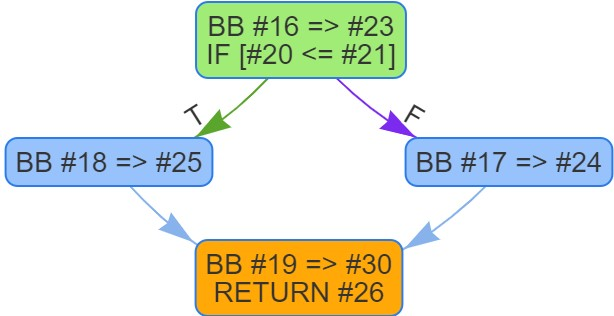
\includegraphics[width=0.5\textwidth]{math-max-cfg}
\caption{Control flow graph of \texttt{java.lang.Math.max(long, long)} }
\label{fig:math-max-cfg}
\end{figure}

Figure \ref{fig:math-max} shows the complete (excluding \texttt{SourceStateInst}) intermediate representation of \texttt{java.lang.Math.max(long, long)}. Dashed lines connect the \texttt{BEGINInst} - \texttt{ENDInst} pairs. Grey lines are the edges of the data flow graph. The orange arrows represent scheduling dependencies while the other arrows (blue, green, violet) are part of the control flow graph.

Moving an instruction to a different basic block can improve the performance of a compiled program greatly \cite{Click95}, but many instructions cannot be moved arbitrarily. For example, consider algorithm \ref{alg:example-floating}. This algorithm has two instructions within the \emph{then}-block of the \emph{if}-statement. The first instruction is a simple constant multiplication. Moving this instruction to the initial basic block (before the \emph{if}), does not alter the semantics of the program. Moving the print instruction to the initial basic block would alter the semantics of the program because \texttt{x} would be printed, even if \texttt{someCondition()} does not hold. The \emph{floating} property of an instruction indicates whether this instruction can be safely moved into different basic blocks. In this example, the multiplication is a floating instruction, and the method call is \emph{non-floating}. This notion is essential for the optimization as \emph{non-floating} instructions need to be moved between basic blocks in some instances.

\begin{algorithm}[H]
\caption{Example of floating instructions}
\label{alg:example-floating}
\If{someCondition()}{
    int x = 10 * 2\\
    println(x)\\
}
\end{algorithm}

\emph{CACAO} uses a technique called \emph{on-stack-replacement}, which enables the virtual machine to replace the current method implementation with a more optimized (or deoptimized) version, while it is active. For this reason, \emph{CACAO} has to be able to translate between the code constructed by the baseline compiler and the code constructed by the second stage compiler. The concept of a \emph{replacement-point} is introduced to enable this complex task. \texttt{SourceStateInst}s, scattered across the intermediate representation, hold the information required by the virtual machine. Some passes (e.g. \texttt{SourceStateAttachmentPass}) rely on the existence of this information. Keeping this information \emph{up-to-date} is a challenge by itself. Further information can be found in \cite{Eisl13}.

\begin{figure}
\center
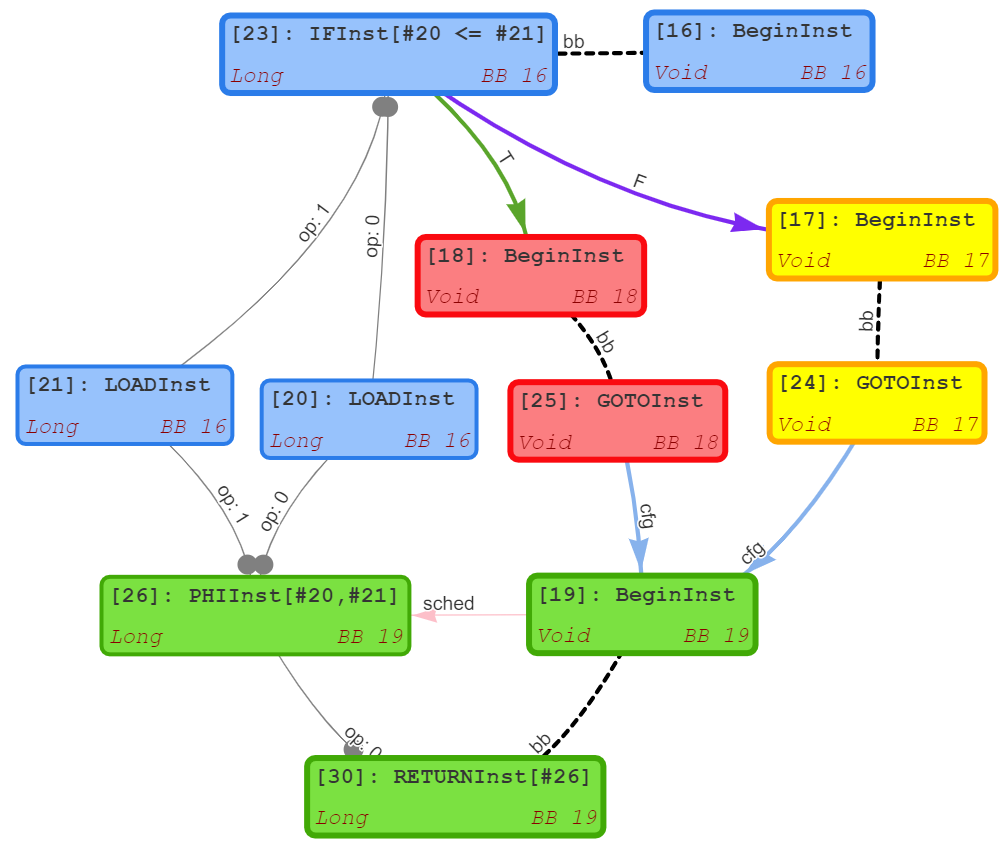
\includegraphics[width=0.75\textwidth]{math-max}
\caption{Intermediate representation of \texttt{java.lang.Math.max(long, long)} (excluding \texttt{SourceStateInst}s) }
\label{fig:math-max}
\end{figure}

\section{Infrastructure}
\label{sec:infrastructure}

\subsection{General}

Currently, \emph{CACAO} lacks an infrastructure to change the \emph{high-level} intermediate representation easily. Therefore, the class \texttt{HIRManipulations} was introduced to encapsulate larger and complex \emph{HIR} transformations, so these can be shared across various passes. The following two operations are required to build the foundation of the inliner. Splitting a basic block at a given instruction and merging two basic blocks, all while keeping the scheduling information correct. This section explains the implementation of these operations.

\subsection{The scheduling graph}
\label{sec:scheduling-graph}

This section gives a more detailed description of \emph{scheduling edges} as they are essential for a complete understanding of the next sections. 

If two instructions are in two different basic blocks, the schedule is already defined in the predecessor and successor relationships of their respective basic blocks. Therefore, scheduling edges are not needed between two instructions which reside in two different basic blocks. Minimizing the \emph{scheduling dependencies} leaving the context of a basic block is done to avoid redundant and possibly inconsistent information, which cannot be considered by the scheduling passes. Note that \emph{scheduling edges} to instructions without an assigned basic block still may be needed. A local scheduling graph only consists of edges with source and target in the same basic block. Therefore, the \texttt{BeginInst} of the basic block is always the root of the local scheduling graph.

Declaring a scheduling dependency from every \emph{state-changing} operation to its last state change ensures correct scheduling between each pair of instructions, thus inductively ensuring correct scheduling for the local scheduling graph. As a result, there is a single path through all \emph{state-changing} operations.

\subsection{Splitting a basic block}

Splitting a basic block with respect to an instruction $I$, is not a trivial task in the intermediate representation used by \emph{Compiler2}. The second stage compiler of \emph{CACAO} uses a graph structure, which does not define any specific ordering of instructions. Therefore a split operation has to analyze the \emph{scheduling} and \emph{data-flow} dependencies to determine which instructions have to follow $I$. Fortunately the \texttt{Instruction} class tracks these edges \emph{bi-directionally}, exposing a \texttt{rdep} and \texttt{user} iterator to other classes. The \texttt{EndInst} of the basic block is a special case as this instruction has to  be moved into the new basic block, whether there are dependencies or not. With the help of the existing capabilities of the \texttt{Instruction} class, the operation is achieved by recursively evaluating the \emph{scheduling} and \emph{data-flow} edges, while moving every depending instruction into the newly created basic block.

This operation breaks some properties of the scheduling graph. Moving one or more \emph{state-changing} instructions to the newly created basic block means breaking the basic block locality of the scheduling graph. The direct successors of $I$ will still declare a dependency on $I$, which still resides in the first basic block. As $I$ was initially the root of the subgraph moved into the second basic block, the new \texttt{BeginInst} will replace $I$ as the new root. All remaining dependencies to the first basic block will be deleted. These two transformations combined ensure that the new \texttt{BeginInst} is the root of the new basic block local scheduling graph. The path through all \emph{state-changing} instructions is preserved. As some instructions use a specific order of their dependencies, it is crucial to replace the dependencies instead of deleting it and adding a new dependency.

This paragraph formally describes the problem of splitting a basic block $A$ into $A$ and $B$ with respect to an instruction $I$. Let $G_A$ and $G_B$ denote the local scheduling graph of the respective basic block. To split the graph, the precondition $I \in G_A$ must hold. The goal is to move all on $I$ depending instructions to $B$, while $I$ remains in the basic block $A$. Because the directed graph may not contain any circles (otherwise scheduling would not be possible), every instruction which is reachable from $I$ by traversing the \emph{reverse scheduling edges} needs to be moved into the new basic block. The same technique can be applied to the \emph{reverse data flow edges} analogously. The union of these two sets then need to be moved into the new basic block. This operation does not create a new \texttt{ENDInst} for the basic block $A$. Handling the creation of the \texttt{ENDInst} is in the responsibility of the compiler pass. The algorithm \ref{alg:split-basic-block} presents a solution to the problem. 

\begin{algorithm}[H]
\caption{Split basic block}
\label{alg:split-basic-block}

\For{Instruction $i$ which depends on $I$}{
    \If{$i \in A$}{
        add\_to\_basic\_block($i$, $B$)\\
        replace\_dependency($i$, $I$, $B$)\\
    }
}
ensure\_endInst\_is\_in($B$)

\For{Instruction $i$ in $B$}{
    \For{Instruction $dep$ which $i$ depends upon}{
        \If{$dep \in A$}{
            remove\_dependency($i$, $B$)\\
        }
    }
}

\end{algorithm}


\subsection{Merging basic blocks}
\label{sec:merge-basic-blocks}

The algorithm described in section \ref{sec:algorithm} can lead to an unnecessary high basic block count, thus creating more compilation overhead in subsequent passes. Furthermore, these superfluous instructions decrease the overall performance of the generated code, as the \emph{Compiler2} does not yet eliminate unnecessary jump instructions. These performance hits are especially a problem if many small methods such as accessors get inlined. To address this issue the \texttt{InliningPass} will coalesce unnecessary basic blocks after inlining a set of \emph{call sites}. The following conditions must hold so that a given basic block $A$ will be merged with a successor $B$.

\begin{itemize}
    \item $A$ must have exactly one successor.
    \item Let $B$ be the only successor of $A$. Then $B$ must only have one predecessor, which is $A$.
\end{itemize}

The algorithm for merging two basic blocks starts at the initial basic block of a method. If all requirements hold for a given basic block $A$, then the algorithm merges the basic blocks by making use of the algorithm \ref{alg:move-instructions} for each invocation. This ensures that the scheduling information, previously given by the different basic blocks, gets preserved.

This paragraph formally describes the problem of appending all instructions of a basic block $B$ to another basic block $A$. Let $G_A$ and $G_B$ denote the local scheduling graph of the respective basic block. Let $F_B$ denote the forest created by deleting the root node of $G_B$. The root node of every tree in $F_B$ needs to declare a scheduling dependency on every leaf of $G_A$. It is sufficient to declare the dependency solely to the leafs of $G_A$ as the scheduling dependency is transitive. The following algorithm presents a solution to the problem.

\begin{algorithm}[H]
\caption{Append instructions}
\label{alg:move-instructions}
\For{Instructions $b \in B$}{
    Set the begin instruction of $A$ as begin instruction of $b$\\

    \If{$b$ has no dependencies to other instructions}{
        \For{Instructions $a$ in $leafs(A)$}{
            Add dependency from $b$ to $a$\\
        }
    }
}
\end{algorithm}

\section{The algorithm}
\label{sec:algorithm}

The algorithm consists of three steps. The \emph{initialization}, the actual \emph{inlining} and the \emph{cleanup} of the actual invoke instructions.

The initialization step creates the algorithm object used for selecting promising \emph{call sites}. For more details on them, see section \ref{sec:heuristics}. For now, only the \emph{Knapsack} heuristic is used. In the future, one may select or parameterize a heuristic at run-time to maximize the benefit for a given scenario.

Before the heuristic can determine a set of invoke instructions to inline, invocations which cannot be inlined need to be discarded. An \texttt{INVOKEInst} will be ignored if one of the following conditions holds for this given call site.

\begin{enumerate}
    \item The instruction is an \texttt{INVOKEINTERFACEInst}. Currently, there is no mechanism implemented to find the implementation in the set of loaded classes.
    \item The instruction is an \texttt{INVOKEVIRTUALInst}, and multiple implementations are loaded.
    \item The instruction is an \texttt{INVOKEVIRTUALInst}, and the method is declared as abstract.
\end{enumerate}

After initialization, the heuristic will produce a set of \emph{call sites} which should be inlined. For each invocation retrieved, the target method is compiled with the second stage compiler. To reduce compilation overhead only the \texttt{SSAConstructionPass}, including all preceding passes, will be run. If the call target is known at \emph{compile-time}, the construction of the \emph{SSA graph} is complete. If the call site could be polymorphic at run-time, a \emph{guard condition} has to be created. This process is described in section \ref{sec:guarded}.

The algorithm splits the basic block in a \emph{pre-call site} and a \emph{post-call site} basic block. Afterwards, all instructions of the target method are moved to the caller method. During this operation, all return instructions need to be transformed into unconditional jump instructions. This is done by replacing the \texttt{RETURNInst} with a \texttt{GOTOInst}. If the target method has a \emph{non-void} return type, \emph{data-flow} edges must be redirected to the operand of the return instruction(s). To handle multiple returns an additional \texttt{PHIInst} is added to the \emph{post-call site} basic block. Special care must be taken when constructing the phi node, as the order of operands needs to be in sync with the order of predecessors on the containing basic block. If the phi node is trivial, it will be replaced by its single operand.

After inlining all instructions from the target method, the \texttt{LOADInst}s of the \emph{callee} will be replaced with the operands known to the \emph{caller}. After the set of \emph{call sites} have been inlined, the actual \texttt{INVOKEInst} will be deleted, if possible.

This algorithm can produce an unnecessary high basic block count if the \emph{callee} consists of a single basic block. To keep the algorithm more straightforward and thus easier to maintain the coalescing of basic blocks is done in a \emph{post-processing} step. The algorithm used for merging basic blocks was already introduced in \ref{sec:merge-basic-blocks}. This operation concludes the inlining algorithm.

\section{Guarded Inlining}
\label{sec:guarded}

This work uses the \emph{guarded inlining} technique already discussed in section \ref{sec:sota-techniques} to support \emph{virtual} method inlining. The guard will be constructed using a \emph{class test} due to its simplicity. This technique does not use any assumptions about the receiving object, but it requires additional instructions. This slows down the code execution, even if there is only a single implementation loaded. The algorithms \ref{alg:guarded-inlining-before} and \ref{alg:guarded-inlining-after} show a simple example of guarded method inlining illustrated in Java.

\begin{algorithm}[H]
\caption{Guarded inlining (before)}
\label{alg:guarded-inlining-before}
obj.virtualCall()
\end{algorithm}

\begin{algorithm}[H]
\caption{Guarded inlining (after)}
\label{alg:guarded-inlining-after}
\eIf{obj.getClass() == ConcreteClass.class}{
    println("Virtual method called!")
}{
    obj.virtualCall()
}
\end{algorithm}

The \emph{SSA graph} of the target method is altered prior to the actual inlining to achieve this transformation. For this reason, a new \texttt{IFInst}, with the \emph{then}-branch set to the guarded code and the \emph{else}-branch pointing to the original \texttt{INVOKEInst}, is created and added to the target method. After this process, the inlining algorithm can continue normally apart from omitting the deletion of the \emph{call site}.

Unfortunately, \emph{Compiler2} does not yet support the invocation of \emph{built-in native} methods. Because \texttt{Java.lang.Object.getClass()} is modelled via a \emph{built-in native} call the guard condition cannot be created correctly at the time of this work. Therefore a simplistic placeholder guard was created. This guard needs to be corrected once the second stage compiler can compile \emph{built-in native}
method invocations. The placeholder is a tautology. Thus, the current implementation should not be used outside of testing scenarios. To circumvent the \emph{built-in native} method problem, one could ship a well-known class \texttt{org.cacaojvm.compiler2.CompilerUtils}, which provides a method to verify the class of the receiver. Furthermore, the need for a method call could be eliminated if the required machine code to obtain the class object is emitted directly. Another approach, which requires extending the compiler backends, introduces a new \emph{HIR} instruction to model the guard condition. This technique comes with the benefit that the \texttt{InlinerPass} is agnostic to whether a \emph{class test} or another strategy (e.g. \emph{method test}) is used to model the guard.

\section{Heuristics}
\label{sec:heuristics}
\subsection{General}

Suitable heuristics are an essential part of an inliner\cite{Prokopec19}, as bad heuristics can result in severe performance degradation. Choosing a good set of instructions is not an easy task, as many factors come into play. The goal of a heuristic is finding a compromise between shorter execution times, longer compilation times and higher memory consumption. The priority between these metrics can vary between different systems and use-cases. One might choose an aggressive heuristic for a server application to benefit from the improved code during subsequent requests. Contrarily, a more passive implementation could be used in client apps to keep the compilation time low, thus making the program feel more responsive to the end-user. During this work, three different heuristics have been implemented.

\subsection{Everything Possible}

The "Everything Possible" heuristic simply inlines every supported invoke instruction it can find. If every instruction is eligible to be inlined, the whole call graph will be flattened into a single method. This heuristic can be used in testing scenarios for the sake of simplicity, but should not be used in production scenarios. Due to the triviality of this heuristic, no further implementation details are given in this work.

\subsection{Limited Breadth First}

The "Limited Breadth First" heuristic takes the same approach as the "Everything Possible" heuristic, but introduces a limit to the inlined instructions. All call sites eligible for inlining will be processed in a FIFO fashion. For each processed \texttt{INVOKEInst} the total instruction count of the next target method is approximated using the byte code size. If the budget would be exceeded by inlining this method, it gets removed from the list of eligible \emph{call sites}. If no \emph{call site} is left, the algorithm completes. This heuristic will not be used in production scenarios as \cite{Steiner07} already suggests, that a more sophisticated heuristic is needed. More advanced heuristics can be compared to this relatively naive approach to determine their effectiveness.

\subsection{Knapsack}

The "Knapsack" heuristic models the problem of choosing a subset of instructions, by reducing it to the well-known \texttt{KNAPSACK} problem. The optimization form of this problem is known to be NP-hard \cite{Scheifler77} but can be approximated in polynomial time by using a greedy algorithm. This algorithm is already implemented in the baseline compiler of CACAO\cite{Steiner07}. The heuristic has, similar to "Limited Breadth First", a cap to the method size. Each \emph{call site} is assigned a benefit ($B$) and a cost($C$). The ratio $\frac{B}{C}$ determines the priority of an instruction. The greedy algorithm selects the instruction with the highest priority until the maximum method size is reached, or no more call sites can be inlined. This approximation to the \texttt{KNAPSACK} problem is rather simple and can produce \emph{non-optimal} solutions, but it can be solved in manageable time in a \emph{just-in-time} compiler.

The tricky part is to find a good approximation for the benefit $B$. The most straightforward implementation sets $B = 1$, thus making the result only depend on the cost of inlining a method. Even though this approach is not optimal in many cases, this approach was implemented due to its simplicity.

\chapter{Evaluation}

\section{General}

The second stage compiler lacks support for some essential language features of \emph{Java}. Therefore running a sophisticated benchmark suite like \emph{SpecJvm} or \emph{DaCapo} is not possible at the moment. Due to these limitations, micro-benchmarks are used similar to \cite{Eisl13}, \cite{Reisinger14} and \cite{Schutzenhofer17}. The source codes of the used benchmarks are given in the appendix.

\section{Methodology}

The optimized version (with the inliner) is compared against the baseline compiler and the non-optimized version of \emph{Compiler2}, by running a set of micro-benchmarks. Each benchmark was run 50 times, and the median of these measurements was used for further evaluation. For this purpose \emph{CACAO} was configured with \texttt{--enable-compiler2}, \texttt{--enable-replacement}, \texttt{--enable-rt-timing} and \texttt{--enable-optimization}. It was compiled with \emph{g++ 9.1.0}.

\subsection{Test System}

All benchmarks were run on a system with an \emph{Intel(R) Core(TM) i7-7700 HQ} running \emph{Ubuntu 16.04.6 LTS} with the kernel \emph{4.19.76-linuxkit}. The operating system was hosted within \emph{Windows 10 1909 (OS Build 18363.719)} using \emph{Docker Engine - Community 19.03.8}.

\subsection{Benchmarks}

The following list shows the benchmarks used for evaluating the inliner.

\begin{itemize}
    \item \texttt{apply-to-array}: Adds the number $6$ to every element of the given array, but the number is derived from a \texttt{getConstant()} invocation. This test aims to show, that subsequent optimizations (in this case constant propagation) yield dramatic speed improvements. Called with $N = 1\_000\_000$.
    \item \texttt{array-times-two}: Multiplies an array by two and saves it into a new array. This test aims to give a basic estimate for the speed improvements. Called with $N = 1\_000\_000$.
    \item \texttt{big-call-graph}: A slightly bigger benchmark. The goal of this benchmark is ultimately to detect some differences between the heuristics. Called with $N = 100\_000$.
    \item \texttt{bubble-sort}: A simple sorting algorithm which should give an estimate on how long the introduced passes take to process a method without any optimization points. No speedup is expected for this benchmark. Called with $N = 1\_000$.
    \item \texttt{categorize-points}: Counts the number of points in each quadrant of a coordinate system. Called with $N = 1\_000\_000$.
    \item \texttt{create-points}: Creates an array of point objects out of two integer arrays. This test aims to asses the speed-up created from constructor inlining. Called with $N = 100\_000$.
    \item \texttt{fibonacci}: Recursive implementation to calculate the \emph{nth} number in the Fibonacci sequence. This test aims to asses the speed-up created from inlining recursive methods. Called with $N = 35$.
\end{itemize}

Benchmarks to measure the effect of guarded inlining are deliberately left out. Due to the current implementation described in section \ref{sec:guarded}, all obtained results would not be comparable to any correct implementation.

\subsection{Key Figures}

The main goal of this work is improving the execution speed of programs. Therefore the primary aspect examined during the evaluation is the total time needed to execute a given program. The total time is obtained with the \texttt{Compiler2TestBase\$TimingResults} class.

As the second stage compiler is a magnitude slower than the baseline compiler \cite{Eisl13}, this value is also broken down into compilation and execution time. With these figures, the effect on total compilation time can be reviewed. The 	measurements were obtained using the timing capabilities of \emph{CACAO}.

To detect code explosion, the total program size has to be considered when evaluating an inliner. As this work uses micro-benchmarks to evaluate the artefact, the memory usage of big applications can only be vaguely estimated. The code size is measured by using the \texttt{ObjectFileWriterPass}. Only the code size of the entry method of each benchmark is evaluated.

\section{Results}

\subsection{micro-benchmarks}

This section will discuss the effect of method inlining in the context of \emph{Compiler2}. Note that these results are agnostic to the used heuristics, as all implemented heuristics will behave exactly the same way, due to the small code size.

Table \ref{tab:benchmarks} displays the median of the obtained measurements, including the relative speed-up in per cent compared to the baseline compiler. These values are visualized in figure \ref{fig:benchmark-runtime}.

\begin{table}
\begin{tabular}{l|c|c|c|c|c}%
    \bfseries Benchmark & \bfseries baseline & \bfseries c2 without & \bfseries c2 with & \bfseries c2 without r. & \bfseries c2 with r.
    \csvreader[head to column names]{data/runtime-speedups.csv}{}
    {\\\hline  \Benchmark & \baseline & \withoutabs & \withabs & \withoutrel$ \,$ \% & \withrel $\,$ \%}
\end{tabular}
\caption{Comparison of implementations. Times are given in $ms$.}
\label{tab:benchmarks}
\end{table}

\begin{figure}
\center
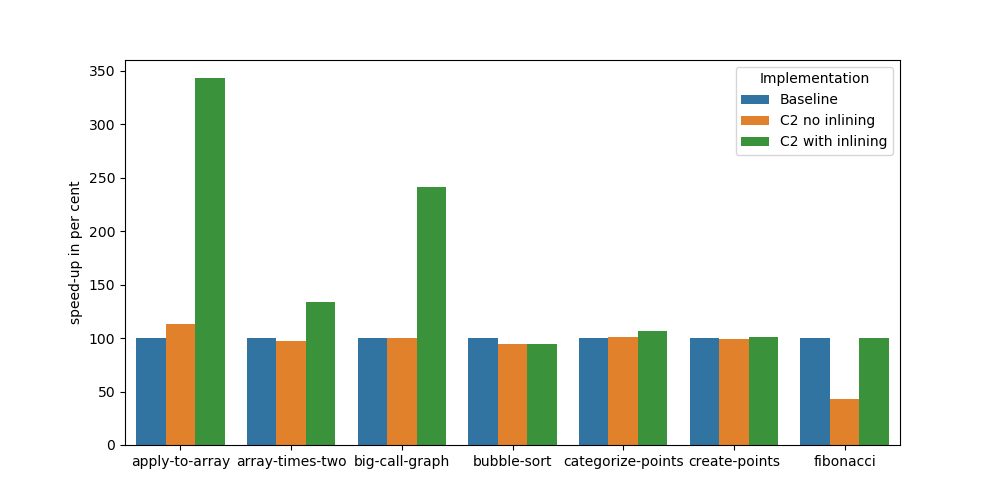
\includegraphics[width=0.8\textwidth]{runtimes-median}
\caption{Relative speed-ups (higher is better)}
\label{fig:benchmark-runtime}
\end{figure}

The median of the absolute time spent in the \texttt{InliningPass} is displayed in table \ref{tab:benchmarks-compilation-time}. Figure \ref{fig:benchmark-compilation-rel} shows the distribution of relative compilation times compared to the total time spent in \emph{Compiler2}\footnote{The benchmark \texttt{bubble-sort} is not included in this graph, because the overhead was virtually zero.}.

\begin{table}[ht]
\begin{tabular}{l|c|c|c|c|c}%
    \bfseries Benchmark & \bfseries total & \bfseries inliner & \bfseries inliner rel. & \bfseries targets & \bfseries targets rel.
    \csvreader[head to column names]{data/compilation-times.csv}{}
    {\\\hline  \Benchmark & \total & \inliner & \relative $\, $ \% & \compileTargets & \compileTargetsRelative $\, $ \%}
\end{tabular}
\caption{Compilation time break-down with the required time to generate the \emph{SSA-Graph} of the call targets. Times are given in $ms$.}
\label{tab:benchmarks-compilation-time}
\end{table}

\begin{figure}[H]
\center
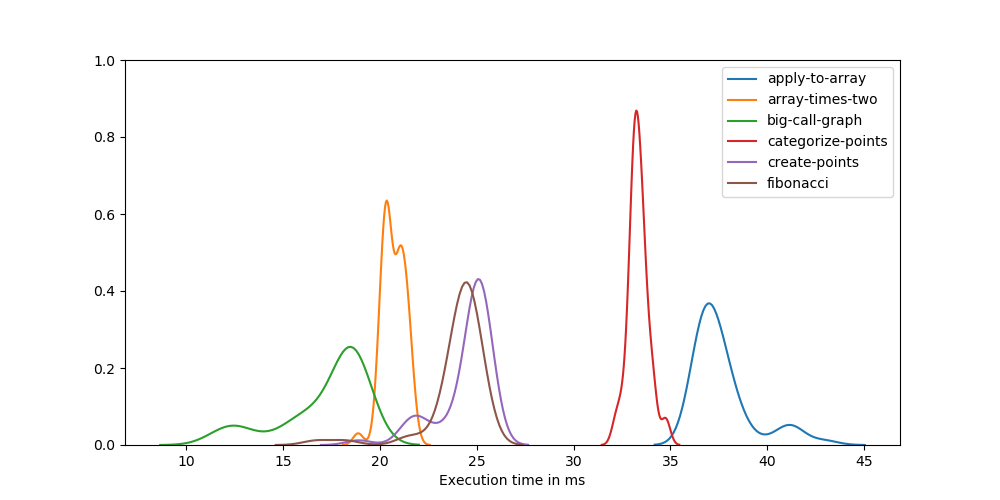
\includegraphics[width=0.8\textwidth]{compilation-times-dist-rel}
\caption{\texttt{InliningPass} relative execution time. This includes the \emph{SSA-Graph} generation of target methods.}
\label{fig:benchmark-compilation-rel}
\end{figure}

\subsection{Heuristics}

This section presents the data gathered from the \texttt{big-call-graph} benchmarks and is used to (vaguely) estimate the effectiveness of the different heuristics. Figure \ref{fig:heuristics-dist} shows the distribution of the absolute running times, while  table \ref{tab:heuristics} shows the median execution time for each heuristic. The measurements were taken without the \texttt{GlobalValueNumberingPass} as this crashed the program in combination with the \texttt{EverythingPossibleHeuristic}. The \texttt{LimitedBreadthFirst} heuristic was initialized with a maximum method size of $100$ instructions, and the \texttt{Knapsack} heuristic was initialized with a budget of $100$ instructions.

\begin{table}[ht]
\center
\begin{tabular}{l|c|c}%
    \bfseries Implementation & \bfseries total time & \bfseries speed up
    \csvreader[head to column names]{data/heuristics.csv}{}
    {\\\hline  \Implementation & \Time & \Speedup $\, $\% }
\end{tabular}
\caption{Total time taken for \texttt{big-call-graph}. Times are given in $ms$.}
\label{tab:heuristics}
\end{table}

\begin{figure}[H]
\center
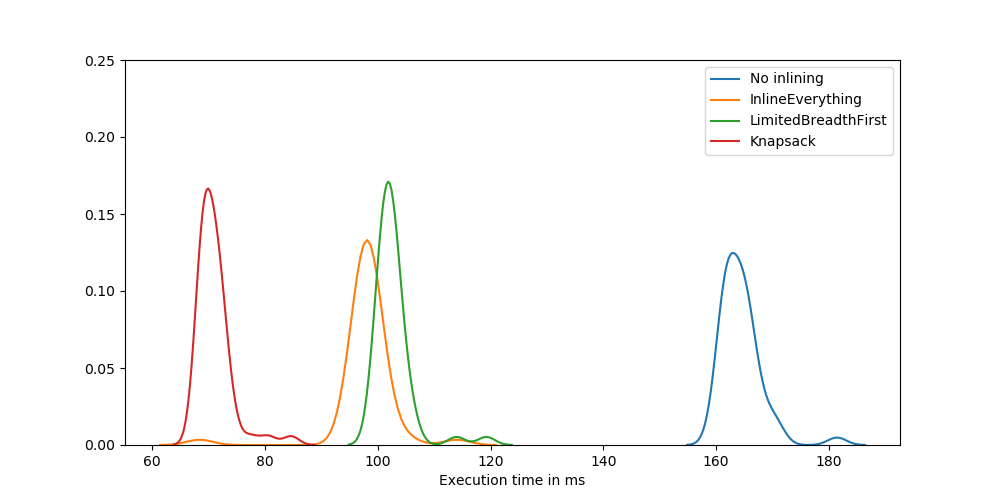
\includegraphics[width=0.8\textwidth]{heuristics-dist}
\caption{Distribution of total execution times in $ms$ per heuristic.}
\label{fig:heuristics-dist}
\end{figure}

Table \ref{tab:codesize} compares the code sizes of the compiled methods. Only the sizes of the entry method are listed.

\begin{table}[ht]
\center
\begin{tabular}{l|c|c}%
    \bfseries Implementation & \bfseries size & \bfseries size rel. \\ \hline  
    No Inlining & $258$ & $100.000 \%$ \\ \hline
    EverythingPossible & $788$ & $305.426 \%$ \\ \hline
    LimitedBreadthFirst & $616$ & $238.759 \%$ \\ \hline
    Knapsack & $720$ & $279.069 \%$ \\ \hline
\end{tabular}
\caption{Code sizes of the entry methods of each benchmark. Sizes are given in \emph{bytes}.}
\label{tab:codesize}
\end{table}

\section{Conclusion}

In this work an inliner for the second stage compiler of the \emph{CACAO VM} was implemented, which can inline methods with statically known targets. Furthermore, a set of heuristics was introduced which guide the inliner in finding promising \emph{call sites}. The guarded adaption of the algorithm was not fully implemented during this work, due to missing capabilities of \emph{Compiler2}. The approach was implemented, while the construction of the \emph{guard} condition was left out.

The results obtained from the benchmarks show promising performance improvements in many cases. The relative duration of the \texttt{InliningPass} ranged from $10$ to $45$ per cent. This increase in compilation time may be too much for a \emph{just-in-time} compiler. A big part of this time is spent with compiling the target methods. These methods could be cached to prevent duplicate compilations of frequently accessed subroutines. The numbers suggest that there is also optimization potential in the actual inlining algorithm, which takes up to $80 \%$ of the total time.

The measured increase in code size is almost $280 \%$ for the \emph{Knapsack} heuristic, which is the default heuristic used by the inliner. These figures suggest that a budget of $100$ may be too big for many real-life applications, due to the drastic increase in code size. Further empirical evaluation needs to be conducted once \emph{Compiler2} is able to run more sophisticated programs.

The evaluation clearly showed the need for an \texttt{InliningPass} in \emph{Compiler2}, and the implementation delivered with this work is a good foundation for a production-ready inliner. The required enhancements for a complete inliner are described in section \ref{sec:future-work}.

\chapter{Future Work}
\label{sec:future-work}

\emph{CACAO} has a complex data structure to allow \emph{on-stack replacement}. Currently, this technique is not supported in combination with this implementation. This mechanism should be implemented in a future work for several reasons. Firstly, the implementation needs to be compatible with other optimizations, which may depend on working deoptimization. Moreover, an assumption based inlining technique could be implemented to eliminate the overhead of a guard condition similar to the \emph{adaptive} inliner used in the baseline compiler. Additionally, correct stack trace recreation needs to be implemented or ported from the baseline compiler.

The current evaluation relies on micro-benchmarks to determine which heuristics improve the overall execution time. All of these code samples are rather small compared to actual \emph{Java} programs. Benchmarks suites should be used to compare the different heuristics to get more accurate measurements and a more thorough understanding of the trade-offs involved, once the second stage compiler supports enough instructions to run them.

Once the second stage compiler is able to re-run passes, one could implement an incremental inlining approach, as suggested by Prokopec19 \emph{et al.} \cite{Prokopec19}. Due to the design choices of \emph{Compiler2}, implementing the possibility to re-run certain stages of the compiler pipeline could prove rather simple. Such a mechanism could enable an implementation of \emph{inlining trials} by adding another pass into the compiler pipeline which evaluates the actual benefits of the expansion.

Currently, inlining is performed on the high-level intermediate representation. Another approach could manipulate the baseline compilers intermediate representation, from which the \emph{SSA-graph} is constructed \cite{Eisl13}. Taking this thought further could result in an approach which uses the inliner of the baseline compiler prior to creating the SSA-graph. Such an approach would drastically limit the flexibility of the implementation but could mitigate the problem with replacement points if the baseline and second stage compiler keep their inlining decisions in sync. If such an approach would be beneficial or even possible needs further investigation.

In this work the \texttt{HIRManipulations} class was introduced to share significant and complex operations on the high-level intermediate representation between different passes. Even though some operations were introduced, there are many possibilities to extend this infrastructure. For example, duplicating a basic block can be used in optimizations such as loop unrolling.

\backmatter


% Add a bibliography.
\printbibliography[title={Bibliography}]

\nocite{Implementation}

\chapter{Appendix}

\section{Benchmarks}
\lstinputlisting[caption=array-times-two]{listings/array-times-two.java}
\lstinputlisting[caption=apply-to-array]{listings/apply-to-array.java}
\lstinputlisting[caption=big-call-graph]{listings/big-call-graph.java}
\lstinputlisting[caption=bubble-sort]{listings/bubble-sort.java}
\lstinputlisting[caption=categorize-points]{listings/categorize-points.java}
\lstinputlisting[caption=create-points]{listings/create-points.java}
\lstinputlisting[caption=fibonacci]{listings/fibonacci.java}
\lstinputlisting[caption=Point class]{listings/Point.java}


\end{document}